%\documentclass{standalone}
%\usepackage{tikz}
%\usepackage{xcolor}
%\usetikzlibrary{fit,positioning}
%
%\usepackage{amsmath}
%\usepackage{amssymb}
%\usepackage{amsfonts}
%\usepackage{mathtools}
%\usepackage{graphicx}
%
%\begin{document}

% ---------------------------------------------------
% Comment above for inclusion in other docs
% ---------------------------------------------------

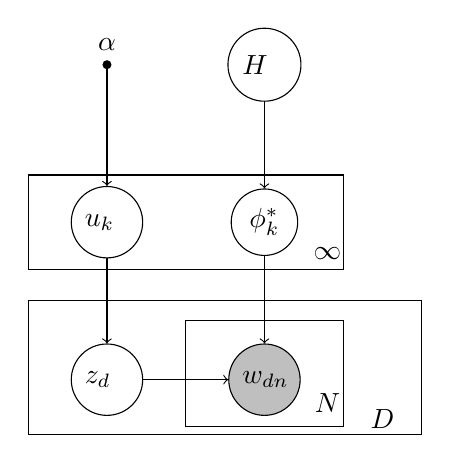
\begin{tikzpicture}
\coordinate (alpha)   at (0,2);
\node (alpha) at (2,4) [circle, draw, inner sep=1pt, fill, label=above:$\alpha$] { };
\node (theta) at (2,2) [circle, draw, text width = 16pt] {$\text{ }u_k$};

\node (b) at (4,4) [circle, draw, text width = 16pt] {$\text{ }H$};
%\node (b) at (2,2) [circle, draw, inner sep=1pt, fill, label=above:$\beta$] { };
\node (z) at (2,0) [circle, draw, text width = 16pt] {$z_d$};

\node (psis) at (4,2) [circle, draw] {$\phi^*_k$};
\node (w) at (4,0) [circle, draw, text width = 16pt, fill=gray!50] {$w_{dn}$};

 
\draw[->] (alpha) -- (theta);
\draw[->] (b.south) -- (psis.north);
 
\draw[->] (theta.south) -- (z.north);
\draw[->] (z.east) -- (w.west);
\draw[->] (psis) -- (w);
 
\draw (1,-.7) rectangle (6.,1);
\draw (3,-.6) rectangle (5,.75);
\draw (1,1.4) rectangle (5,2.6);
 
\node at (5.5,-.5) {$D$};
\node at (4.8,-.3) {$N$};
\node at (4.8,1.6) {$\infty$};
  
\end{tikzpicture}

% ---------------------------------------------------
% Comment below for inclusion in other docs
% ---------------------------------------------------

%\end{document}